\documentclass{report}
\usepackage[style=numeric]{biblatex}
\usepackage{multirow}
\usepackage{graphicx}
\addbibresource{references.bib}
\graphicspath{ {../assets/} }

\def\frontmatter{%
    \pagenumbering{roman}
    \setcounter{page}{1}
    \renewcommand{\thesection}{\Roman{section}}
}%

\def\mainmatter{%
    \pagenumbering{arabic}
    \setcounter{page}{1}
    \setcounter{section}{0}
    \renewcommand{\thesection}{\arabic{section}}
}%

\def\backmatter{%
    \setcounter{section}{0}
    \renewcommand{\thesection}{\Alph{section}}
}%

\title{Progress Report 1 \\ Building new AI applications for a distributed AI serving system}
\author{Waqas Ali\\{\small Supervisor: Dr. Heming Cui}\\{\small Mentor: Shixiong Zhao}}
\date{\today}
 
\begin{document}
\frontmatter
\maketitle

\addcontentsline{toc}{chapter}{Abstract}
\begin{abstract}
abstract-text
\end{abstract}

\tableofcontents

\addcontentsline{toc}{chapter}{\listfigurename}
\listoffigures

\addcontentsline{toc}{chapter}{\listtablename}
\listoftables

\mainmatter

\chapter{Introduction}

\section{Background}
Artificial intelligence is an area of computer science which focuses on granting machines the ability to act intelligently \cite{McCarthy2007}. It's a vast field with limitless applications and each application has its own unique solution. Machine learning, specifically, is a subset of artificial intelligence which learns from data. \cite{Mitchell1997} Nowadays we see artificial intelligence everywhere from spam filters \cite{Androutsopoulos2000} to movie recommendations \cite{lekakos2008hybrid} to virtual assistants to self-driving.

Customers are demanding smarter and smarter capabilities in their machines which leads to its own set of software development challenges; Nvidia summarises them with the PLASTER \cite{Teich2018} framework:
\begin{itemize}
  \item Programmability
  \item Latency
  \item Accuracy
  \item Size of Model
  \item Throughput
  \item Energy Efficiency
  \item Rate of Learning
\end{itemize}

These challenges arise during the development lifecycle of any machine learning application. A machine learning application has two main stages:
\begin{enumerate}
  \item Training (Learning from data)
  \item Inference (Given an input, predicting an output)
\end{enumerate}

For example, for virtual assistants, training the voice recognition model involves exposing the program to hundreds of voice recordings and letting it figure out what sounds correspond to which words. Inference, however, is inputting a new voice recording and transcribing it using the trained voice recognition model.

End-users of machine learning applications are only concerned with inference and they expect real-time response.

\begin{figure}
  \centering
  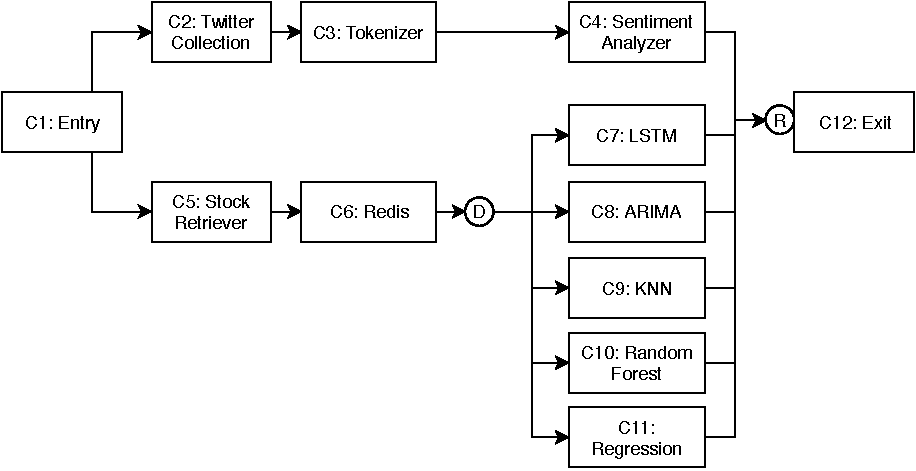
\includegraphics[width=\textwidth]{StockPriceServiceBasic.pdf}
  \caption{Inference pipeline of a basic stock price prediction service. C2 and C5 are data retrievers. C6 is a caching layer. C7, C8, C9, C10 \& C11 are ML models which compete against each other. C4 is a sentiment analyzer whose results are taken into account for price prediction.}
  \label{fig:StockPriceServiceBasic}
\end{figure}

As AI application pipelines get complex, inference can take a long time. For instance, a stock price prediction service (Figure \ref{fig:StockPriceServiceBasic}) involves several steps. On a monolith architecture, all tasks have to be done sequentially (even if they are independent of each other). This could take a long time and hence increase the latency. Moreover, until all tasks for a specific request have finished, processing for a new request cannot be started. Thus, the service cannot handle high number of requests in a given time period i.e. throughput.

This is exactly the kind of situation where a distributed system could shine. By deploying several servers which could independently accomplish the pipeline tasks above, theoretically we can improve the latency and throughput of an AI application (concerns which were highlighted in the PLASTER framework \cite{Teich2018}).

\section{Objective}
The project's aim is to improve latency and throughput of AI applications by implementing and deploying them on a distributed system. As a proof of concept, an AI application will be chosen which has a complex inference pipeline and it will be developed on a distributed system.

To prove that a distributed architecture can indeed improve latency and throughput, performance will be compared across systems of various specifications:
\begin{enumerate}
  \item 1 node for n tasks (baseline)
  \item less than n nodes for n tasks
  \item n nodes for n tasks (optimum)
\end{enumerate}

\chapter{Methodology}
\begin{enumerate}
  \item Choose AI Application i.e. Smart Driving, Stock Price Prediction, etc.
  \item Develop and run basic inference pipeline on a monolith architecture.
  \item Convert the pipeline to run using RPC (remote procedure call) on one server.
  \item Deploy the above on multiple servers.
  \item Devise a method to programmatically instantiate cloud resources and deploy model.
  \item Compare latency and throughput of model on distributed systems of various specifications.
\end{enumerate}

\chapter{Current Status}
Current status. Evaluation of progress.

\chapter{Schedule}
\begin{table}[h!]
  \begin{center}
    \caption{Project Schedule}
    \label{tab:table1}
    \begin{tabular}{ |l|l| } 
      \hline
      \multicolumn{2}{|c|}{2019} \\ \hline
      \multirow{2}{*}{October} & Choose \& Design AI application to work on \\
       & Develop a basic inference pipeline on a monolithic architecture \\ \hline
      November & Convert pipeline to work on a distributed system using RPC \\ \hline
      December & Manually deploy pipeline to distributed architecture on cloud \\ \hline
      \multicolumn{2}{|c|}{2020} \\ \hline
      \multirow{3}{*}{January} & Programmatically instantiate cloud resources and deploy model \\
       & First Presentation \\
       & Detailed interim report \\ \hline
      February     & Vary deployments by cloud resources and measure latency/throughput on each  \\ \hline
      March     & Enhance AI inference pipeline by adding more steps  \\ \hline
      \multirow{3}{*}{April} & Finalize implementation \\
       & Final Presentation \\
       & Final Report \\ \hline
      \end{tabular}
  \end{center}
\end{table}

\chapter{Limitations and Potential Difficulties}
Limitations and Potential Difficulties

\chapter{Conclusion}
Conclusion

\backmatter

\addcontentsline{toc}{chapter}{Bibliography}
\printbibliography

\end{document}